\section{Illustrative Example} \label{sec:expl}

We present a toy example to illustrate the lower bound feasibility and bound tightening procedures as well as the upper bound approximation method.
We take the problem data as follows.

\[
A=
\begin{bmatrix}
  -1 & \p 0  \\ 
\p 1 & \p 0  \\  
\p 0 & -1 \\
\p 0 & \p 1  
\end{bmatrix},%
~
\vb =
\begin{bmatrix}
  -0.5  \\ 
\p 3 \\  
  -0.5 \\
\p 3  
\end{bmatrix}, %
~
Q_1=
\begin{bmatrix}
  1 & 0  \\ 
  0 & 0  
\end{bmatrix},%
~
Q_2=
\begin{bmatrix}
  0 & 0  \\ 
  0 & 1  
\end{bmatrix},%
~
L=
\begin{bmatrix}
  1 & -3  \\ 
  2 & -1  
\end{bmatrix}, %
~\mbox{ and }
\vu^*=
\begin{bmatrix}
  -2  \\ 
\p 4   
\end{bmatrix}.%
\]
%
These components of data correspond to the following quadratic system.
\[
F(\vx) =
\begin{bmatrix}
  x_1^2 + ~~x_1 - x_2 \\
  x_2^2 +  2x_1 - x_2
\end{bmatrix}
=
\begin{bmatrix}
    -2 \\
    \p 4
\end{bmatrix}
\hspace*{0.15in}
\text{ with }
\hspace*{0.15in}
\Omega_{\vx} = \left\{ \vx ~\big\vert~
\begin{bmatrix}
  0.5 \\
  0.5
\end{bmatrix}
\leq 
\begin{bmatrix}
  x_1 \\
  x_2
\end{bmatrix}
\leq
\begin{bmatrix}
  3 \\
  3
\end{bmatrix}
\right\}.
\]

Running the Outer Bound Procedure B (\cref{eq:OPTfeasOutRelaxb}) gives an upper bound on the robustness margin of $2.63462$.
Running the feasibility procedure results in an lower bound on the robustness margin of $1.20454$\delete{BK: Which procedure---LP or MIP?}, while the bound tightening yields a lower bound of $1.706649$. 

We illustrate $F(\Omega_{\vx})$ with $\vu^*$ in \cref{fig:FOmega}.
Notice that the bound tightening procedure produces a better lower bound approximation as theoretically predicted.
All procedures were run using their most relaxed forms.\delete{BK: What do you mean by this last sentence exactly?}

\delete{BK: Also, what is the center of the boxes? May be list that solution as well.}

\begin{figure}[htp!]
  \begin{center}
    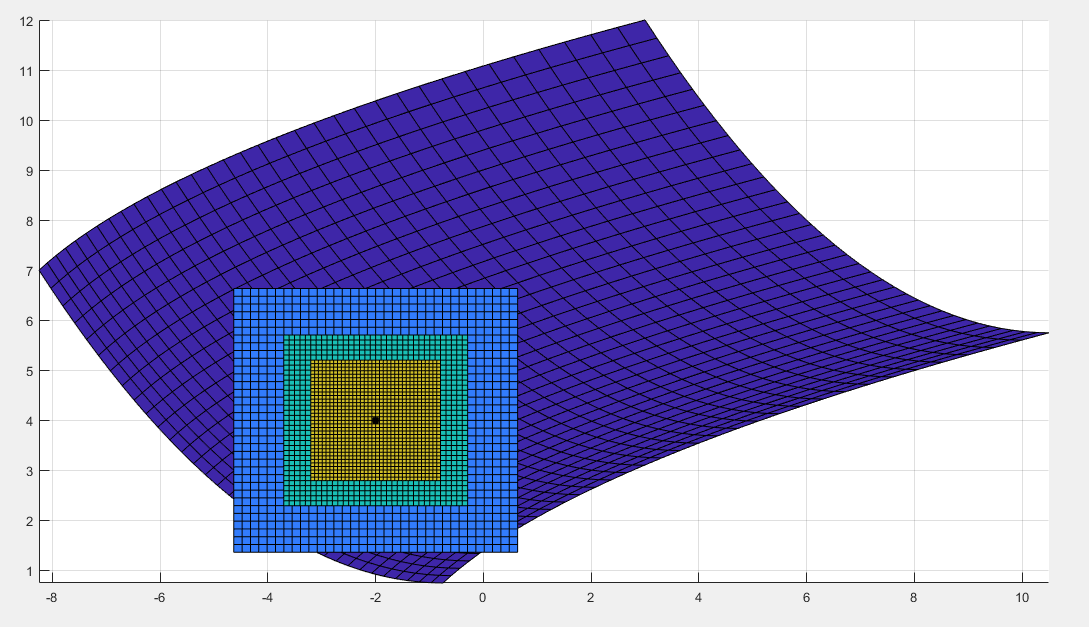
\includegraphics[scale=0.45]{Figures/newex} % {Figures/Rfeas}
  \end{center}
  \caption{\label{fig:FOmega}
    Illustration of $F(\Omega_x)$ (dark blue surface), $\vu^*$, and $\Omega_{u^*}$ with radii given by the upper bound procedure (light blue box), bound tightening procedure (turquoise box), and feasibility procedure (yellow box).
  }
\end{figure}


